\chapter{Equation of State, Radiation, and Vacuum Energy}

\lectureoverview{The history of a homogeneous universe is largely the history of its scale factor \(a(t)\). Friedmann's equation supplies the geometry, but the material equation of state tells us how the energy density changes while space expands. We first derive \(\rho\propto a^{-3(1+w)}\) from work done by a fluid, then obtain \(P=\rho/3\) for radiation by counting photon momentum transfer, and finally identify vacuum energy by \(P=-\rho\). Positive vacuum energy produces de Sitter expansion; curvature and the sign of the cosmological constant produce bounce and recollapse solutions that can be read as simple mechanical systems.}

\section{The Scale Factor and the Missing Material Law}

Let us first recover where we are going. Within the homogeneous and isotropic approximation, the main cosmological history is encoded in one function, \(a(t)\). Knowing that function does not answer every question about the universe, but it determines distances, expansion rates, and the sequence of large-scale eras. The purpose of this lecture is not yet to establish those eras observationally. It is to derive, from basic physics, the equations of state that make the models possible. \lecturetimestamp{00:00:09--00:01:39}

Two benchmark models have already appeared:
\begin{equation}
a(t)\propto t^{2/3}
\qquad\text{(matter domination)},
\end{equation}
and
\begin{equation}
a(t)\propto t^{1/2}
\qquad\text{(radiation domination)}.
\end{equation}
Neither law is exact for all times. Radiation gives the useful early-time approximation and matter the later intermediate one; vacuum energy eventually changes the late-time behavior again. The immediate question is not how observations reveal these eras, but what distinguishes the corresponding right-hand sides of Friedmann's equation. \lecturetimestamp{00:01:39--00:02:49}

\begin{figure}[htbp]
\centering

\includegraphics[width=0.72\textwidth]{lecture_05_figure_02.png}
\caption{The reviewed scale-factor power laws and the newly introduced density symbol. This is a transitional board state rather than a completed derivation.}
\label{fig:c05-review-board}
\lectureframe{00:03:18.380}
\end{figure}

The missing bridge is the equation of state. It determines how the energy density on the right-hand side of Friedmann's equation changes with the scale factor. The two benchmark laws are
\begin{equation}
\rho_{\text{matter}}=\frac{\rho_0}{a^3},
\qquad
\rho_{\text{rad}}=\frac{\rho_0}{a^4}.
\label{eq:c05-benchmark-densities}
\end{equation}
Matter dilutes with volume, and volume scales as \(a^3\). Radiation falls with one additional power of \(a\). We want to understand both rules as consequences of the relation between pressure and energy density. \lecturetimestamp{00:02:49--00:04:31}

\section{From Pressure to the Density-Scaling Law}

An equation of state may generally involve density, pressure, temperature, and other variables. For the cosmological components considered here, adopt the useful constant-\(w\) form
\begin{equation}
P=w\rho,
\label{eq:c05-eos}
\end{equation}
where \(w\) characterizes the fluid. The board uses an uppercase \(W\); we use the conventional lowercase \(w\). This linear form covers the important cases below, but it is a simplifying ansatz rather than a law obeyed by every possible fluid. \lecturetimestamp{00:04:31--00:05:39}

For nonrelativistic matter, energy density is dominated by rest energy. If \(n\) is the number density and \(m\) the particle mass, then schematically
\begin{equation}
\rho\simeq nmc^2.
\end{equation}
The factor \(c^2\) makes even a small rest mass an enormous reservoir of energy; complete annihilation of a dust grain would release a macroscopic amount. Pressure, by contrast, is produced by momentum transfer when particles strike a wall and is of order \(nmv^2\). A bowling ball transfers more momentum than a ping-pong ball, but for a cold gas every relevant speed satisfies \(v\ll c\). Hence
\begin{equation}
\frac{P}{\rho}\sim\frac{v^2}{c^2}\ll1,
\qquad
w\simeq0.
\label{eq:c05-dust-eos}
\end{equation}
Radiation moves at \(c\), so it will not share this approximation. We shall derive its value of \(w\) rather than assume it. \lecturetimestamp{00:05:39--00:08:46}

We now need a general machine that turns equation~\eqref{eq:c05-eos} into a scaling law for \(\rho\). A laboratory box is enough. Galaxies cannot literally be placed in a box, but after coarse-graining they behave as particles, and the relation between energy and pressure can be derived locally. \lecturetimestamp{00:08:46--00:09:44}

\begin{figure}[htbp]
\centering

\includegraphics[width=0.86\textwidth]{lecture_05_figure_03.png}
\caption{The equation of state, reviewed density scalings, and the thermodynamic box on one board. The lecturer obscures part of the earlier writing, so the image is used for layout and visible equations rather than as a complete transcription.}
\label{fig:c05-box-board}
\lectureframe{00:13:39.612}
\end{figure}

The left side of the board carries the reviewed cosmological scalings; the right starts the box argument. Read together, the visible content connects
\begin{equation}
\rho_{\text{matter}}=\frac{\rho_0}{a^3},
\qquad
\rho_{\text{rad}}=\frac{\rho_0}{a^4},
\qquad
P=w\rho.
\end{equation}
Our task is to derive the two density laws from the equation of state.

One wall has area \(A\). Move it outward by \(dx\), so
\begin{equation}
dV=A\,dx.
\end{equation}
Pressure is force per area, so the force on the wall is \(PA\). The gas does work \(PA\,dx=P\,dV\), and the energy remaining inside decreases. \lecturetimestamp{00:09:44--00:12:14}
\begin{equation}
dE=-P\,dV.
\label{eq:c05-work-law}
\end{equation}
\begin{figure}[htbp]
\centering
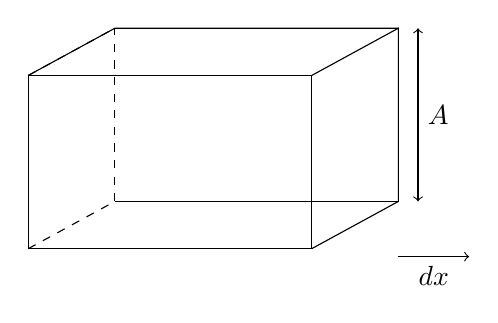
\begin{tikzpicture}[scale=1.0]
\draw (0,0) -- (3.6,0) -- (3.6,2.2) -- (0,2.2) -- cycle;
\draw (3.6,0) -- (4.7,0.6) -- (4.7,2.8) -- (3.6,2.2);
\draw (0,2.2) -- (1.1,2.8) -- (4.7,2.8);
\draw (1.1,0.6) -- (4.7,0.6);
\draw[dashed] (0,0) -- (1.1,0.6);
\draw[dashed] (0,2.2) -- (1.1,2.8);
\draw[dashed] (1.1,0.6) -- (1.1,2.8);
\draw[<->] (4.95,0.6) -- (4.95,2.8);
\node[right] at (4.95,1.7) {\(A\)};
\draw[->] (4.7,-0.1) -- (5.6,-0.1);
\node[below] at (5.15,-0.1) {\(dx\)};
\end{tikzpicture}
\caption{A clean reconstruction of the thermodynamic box, with face area \(A\) and displacement \(dx\).}
\label{fig:c05-box-redraw}
\end{figure}

The total energy is
\begin{equation}
E=\rho V.
\end{equation}
Differentiating gives
\begin{equation}
d(\rho V)=\rho\,dV+V\,d\rho.
\end{equation}
Substitution into equation~\eqref{eq:c05-work-law} gives
\begin{equation}
\rho\,dV+V\,d\rho=-P\,dV.
\end{equation}
Insert \(P=w\rho\):
\begin{equation}
V\,d\rho=-(1+w)\rho\,dV.
\end{equation}
The result is preliminary to the useful equation, but not quite there. Divide by \(\rho V\). \lecturetimestamp{00:12:14--00:15:19}
\begin{equation}
\frac{d\rho}{\rho}=-(1+w)\frac{dV}{V}.
\end{equation}
\begin{figure}[htbp]
\centering

\includegraphics[width=0.78\textwidth]{lecture_05_figure_04.png}
\caption{The separated density-volume equation and the beginning of the logarithmic integration. The complete right-hand side is reconstructed from the preceding algebra, not from hidden pixels.}
\label{fig:c05-log-board}
\lectureframe{00:15:35.600}
\end{figure}

The frame shows the separated equation and the beginning \(\log\rho=\). Complete the integration directly:
\begin{equation}
d(\log\rho)=-(1+w)\,d(\log V),
\end{equation}
so that
\begin{equation}
\log\rho=-(1+w)\log V+\text{const.}
\end{equation}
Exponentiating,
\begin{equation}
\rho\propto V^{-(1+w)}.
\end{equation}
This is the density-volume law.

Return now from the box to cosmology. Moving only one wall was a convenient derivation, not an anisotropic assumption. Expanding all three directions uniformly gives the same work relation, and a comoving volume scales as
\begin{equation}
V\propto a^3.
\end{equation}
Therefore
\begin{equation}
\boxed{\rho\propto a^{-3(1+w)}}.
\label{eq:c05-density-scaling}
\end{equation}
In \(d\) spatial dimensions the exponent \(3\) would become \(d\); the rest of the argument is unchanged. \lecturetimestamp{00:15:19--00:17:53}

\section{First Applications: Matter and Radiation}

We can now recover the review formulas as consequences rather than assumptions.

For nonrelativistic matter we take
\begin{equation}
w=0.
\end{equation}
Then
\begin{equation}
\rho\propto a^{-3},
\end{equation}
which is exactly the matter-dilution law.

For radiation, provisionally take
\begin{equation}
w=\frac13.
\end{equation}
If this is correct, then
\begin{equation}
\rho\propto a^{-3(1+1/3)}=a^{-4}.
\end{equation}
The extra inverse power is therefore equivalent to \(w=1/3\). The unresolved step is to derive that value from photon physics. \lecturetimestamp{00:17:53--00:19:11}

\section{Why Radiation Pressure Is One Third of Its Energy Density}

Radiation may be described as electromagnetic waves or as massless particles. Use photons and compute the pressure of a photon gas in a box. The box is drawn in two dimensions, but the gas and its angular distribution are three-dimensional. The photons move at the speed of light and bounce elastically from the provisional walls. \lecturetimestamp{00:19:11--00:20:44}

For the moment, pretend all photons have the same energy \(\epsilon\). This simplification will disappear when the contributions from different energies are added. Let \(\vec{\pi}\) be a photon momentum vector; the usual \(p\) is avoided because \(P\) already denotes pressure. A massless particle obeys the following relations. \lecturetimestamp{00:20:44--00:25:49}
\begin{equation}
\epsilon=c\,\pi,
\end{equation}
with \(\pi=|\vec{\pi}|\). In the units used in the lecture, \(c=1\), so
\begin{equation}
\epsilon=\pi.
\end{equation}
If \(\nu\) is the photon number density, then the energy density is
\begin{equation}
\rho=\epsilon\,\nu.
\end{equation}
Let the \(x\)-axis be normal to one wall. During a short interval \(\Delta t\), a photon moving at angle \(\theta\) to that normal reaches the wall only if it starts within a slab of thickness
\begin{equation}
\Delta x=\Delta t\cos\theta.
\end{equation}
If it reflects, its \(x\)-component of momentum reverses sign, so the momentum transferred to the wall is
\begin{equation}
\Delta \pi_x=2\epsilon\cos\theta.
\end{equation}
Force is momentum transfer per unit time, so one hit contributes \(\Delta \pi_x/\Delta t\). The number of photons in the slab is \(\nu A\Delta x\), but only half of them move toward the wall, so the relevant number is \(\tfrac12 \nu A\Delta x\). Dividing the total force by the wall area \(A\), we find
\begin{align}
P(\theta)
&=
\frac{1}{A}
\left(\frac{2\epsilon\cos\theta}{\Delta t}\right)
\left(\frac12 \nu A\Delta x\right) \\
&=
\epsilon\nu\cos\theta\frac{\Delta x}{\Delta t} \\
&=
\epsilon\nu\cos^2\theta \\
&=
\rho\cos^2\theta.
\end{align}
The result depends on angle because it is only the contribution from photons traveling in one direction. \lecturetimestamp{00:25:52--00:34:57}

\begin{figure}[htbp]
\centering
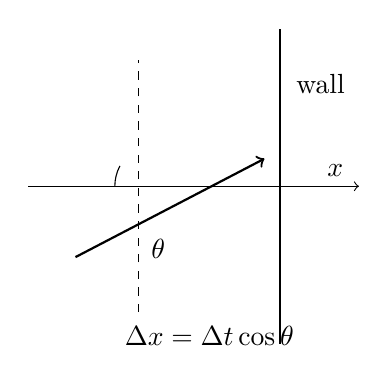
\begin{tikzpicture}[scale=1.0]
\draw[thick] (0,0) -- (0,4);
\draw[->] (-3.2,2) -- (1.0,2);
\node[above] at (0.7,2) {\(x\)};
\draw[dashed] (-1.8,0.4) -- (-1.8,3.6);
\node[below] at (-0.9,0.35) {\(\Delta x=\Delta t\cos\theta\)};
\draw[->,thick] (-2.6,1.1) -- (-0.2,2.35);
\node[below] at (-1.55,1.45) {\(\theta\)};
\draw (-2.1,2) arc[start angle=180,end angle=152,radius=0.55];
\node[right] at (0.08,3.3) {wall};
\end{tikzpicture}
\caption{Transcript-backed reconstruction of the photon-pressure geometry.}
\label{fig:c05-photon-pressure}
\end{figure}

Average over the isotropic distribution. Let \(\mathbf n=(n_x,n_y,n_z)\) be the unit vector along a photon's direction. Then
\begin{equation}
n_x=\cos\theta,
\qquad
n_x^2+n_y^2+n_z^2=1.
\end{equation}
In an isotropic gas, the averages of \(n_x^2\), \(n_y^2\), and \(n_z^2\) are equal. Averaging the identity above,
\begin{equation}
\langle n_x^2\rangle+\langle n_y^2\rangle+\langle n_z^2\rangle=1,
\end{equation}
and by symmetry each term is the same, so
\begin{equation}
\langle n_x^2\rangle=\langle \cos^2\theta\rangle=\frac13.
\end{equation}
Therefore
\begin{equation}
P=\rho\langle \cos^2\theta\rangle=\frac{\rho}{3}.
\end{equation}
So the radiation equation of state is
\begin{equation}
P=\frac13\rho,
\qquad
w=\frac13.
\end{equation}
The factor \(1/3\) is the number of spatial directions sharing the squared unit vector. In \(d\) isotropic spatial dimensions, the same argument would give \(\langle n_x^2\rangle=1/d\). This completes the microscopic derivation promised at the start. \lecturetimestamp{00:34:59--00:39:08}

\subsection{Questions That Test the Radiation Argument}

\begin{classroomqa}
\audiencequestion{Do all photons need to have the same energy?}
\lecturerresponse{No. Perform the calculation separately in each energy interval. Every interval contributes pressure equal to one third of its own energy density, so summing over the spectrum preserves \(P=\rho/3\). The equal-energy assumption only kept the notation short. \lecturetimestamp{00:39:08--00:39:36}}
\end{classroomqa}

\begin{classroomqa}
\audiencequestion{Would absorbing black walls give the same answer as perfect mirrors, and what is the wall in empty space?}
\lecturerresponse{A black wall in thermal equilibrium absorbs and re-emits radiation, producing the same average momentum balance. Cosmological space has no literal wall; the surface is an imagined boundary. For every photon that crosses outward, isotropy supplies an average compensating flux inward, so the local momentum-flow calculation is unchanged. The classroom radiation is chiefly the thermal cosmic microwave background, for which this equilibrium picture is especially natural. \lecturetimestamp{00:39:37--00:41:19}}
\end{classroomqa}

\begin{classroomqa}
\audiencequestion{Do quantum statistics change \(P=\rho/3\)?}
\lecturerresponse{No. Bose statistics determine how photons populate the available modes and therefore determine the spectrum and total \(\rho\), but the isotropic stress of massless particles remains one third of that energy density. \lecturetimestamp{00:41:51--00:42:02}}
\end{classroomqa}

\begin{classroomqa}
\audiencequestion{What if photons scatter from one another?}
\lecturerresponse{Ordinary photon-photon scattering is extremely weak, so its correction here is negligible. At sufficiently high temperature and density, collisions can create electron-positron pairs and change the effective particle content and equation of state. That is a real effect, but it belongs to a much hotter regime than the one used in this argument. \lecturetimestamp{00:42:02--00:43:08}}
\end{classroomqa}

\begin{classroomqa}
\audiencequestion{What happened to the wall area \(A\)?}
\lecturerresponse{The intermediate product is the force from one photon times the number striking the wall, and that number is proportional to \(A\). Pressure is force divided by area, so the final division cancels \(A\). Calling the intermediate expression pressure too early was the board omission; restoring the force-to-pressure step repairs it. \lecturetimestamp{00:43:11--00:44:01}}
\end{classroomqa}

\section{Negative Pressure and the Meaning of Tension}

Up to now, particles have struck the walls and pushed them outward. That picture naturally produces positive pressure, but it does not exhaust the possibilities.

\begin{classroomqa}
\audiencequestion{Can energy density itself be negative?}
\lecturerresponse{Quantum theory permits negative energy densities in restricted circumstances, and a cosmological constant can formally have either sign. Such cases require care and are not the immediate starting point. The more familiar doorway is negative \emph{pressure}, which can occur even while the energy density is positive. \lecturetimestamp{00:44:25--00:44:59}}
\end{classroomqa}

\begin{classroomqa}
\audiencequestion{How can pressure be negative?}
\lecturerresponse{In a one-dimensional world, a box is a line interval. Freely moving particles bounce from its ends and push outward, giving positive pressure. Connect the ends instead by a stretched string or spring. Pulling the ends apart makes the spring pull them inward. That inward force is tension, the one-dimensional model of negative pressure. \lecturetimestamp{00:45:04--00:46:31}}
\end{classroomqa}

\begin{figure}[htbp]
\centering
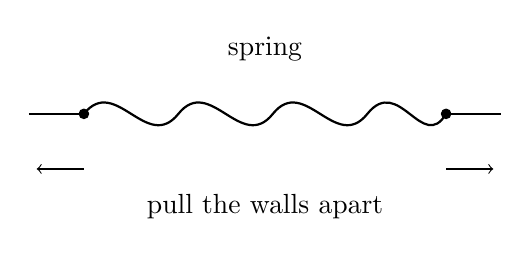
\begin{tikzpicture}[scale=1.0]
\draw[thick] (-3,0) -- (-2.3,0);
\draw[thick] (2.3,0) -- (3,0);
\draw[fill] (-2.3,0) circle (0.06);
\draw[fill] (2.3,0) circle (0.06);
\draw[thick] (-2.3,0)
.. controls (-1.9,0.5) and (-1.5,-0.5) .. (-1.1,0)
.. controls (-0.7,0.5) and (-0.3,-0.5) .. (0.1,0)
.. controls (0.5,0.5) and (0.9,-0.5) .. (1.3,0)
.. controls (1.7,0.5) and (2.0,-0.5) .. (2.3,0);
\draw[->] (-2.3,-0.7) -- (-2.9,-0.7);
\draw[->] (2.3,-0.7) -- (2.9,-0.7);
\node[below] at (0,-0.9) {pull the walls apart};
\node[above] at (0,0.55) {spring};
\end{tikzpicture}
\caption{A one-dimensional spring as an analogy for negative pressure.}
\label{fig:c05-tension}
\end{figure}

The work bookkeeping reverses accordingly. Expansion lets a positive-pressure gas do work and lose internal energy. Pulling outward against tension stores energy in the spring. More generally, attractive constituents can pull one another and the boundary inward. Thus a system may have \(\rho>0\) and \(P<0\), giving \(w<0\), without any contradiction. This possibility is central because vacuum energy has precisely that sign pattern. \lecturetimestamp{00:46:31--00:47:57}

\section{Vacuum Energy and the Cosmological Constant}

Vacuum energy is assigned to empty space itself. Quantum field theory motivates it through the zero-point motion of the harmonic oscillators associated with field modes, but its macroscopic description does not require us to solve that microscopic problem. The defining property is that empty space has the same energy density wherever and however large a region is chosen. \lecturetimestamp{00:47:57--00:50:05}
\begin{equation}
\rho=\rho_0=\text{const.}
\label{eq:c05-vacuum-density}
\end{equation}
If a region of volume \(V\) contains only vacuum energy, then the total energy in that region is
\begin{equation}
E=\rho_0 V.
\end{equation}
\begin{classroomqa}
\audiencequestion{Does a box change the vacuum density by restricting the allowed field modes?}
\lecturerresponse{The total energy in a finite region is smaller than the energy in all of space because the region has smaller volume; the bulk density \(\rho_0\) remains the same. Real boundaries can change mode energies and produce the Casimir effect, but that correction matters when separations are comparable to the relevant wavelengths. It is not the large-scale vacuum density used in cosmology. \lecturetimestamp{00:50:06--00:51:25}}
\end{classroomqa}

Introduce
\begin{equation}
\Lambda=\frac{8\pi G}{3}\rho_0.
\label{eq:c05-lambda-definition}
\end{equation}
This definition absorbs the combination that appears in Friedmann's equation. The inverse relation is
\begin{equation}
\rho_0=\frac{3\Lambda}{8\pi G}.
\end{equation}
The parameter \(\Lambda\) is the cosmological constant. A positive nearly constant component driving late acceleration is commonly called dark energy. \lecturetimestamp{00:51:25--00:53:45}

The scale-factor dependence is already settled, so run the box argument backward to discover its pressure. Since \(d\rho_0=0\),
\begin{equation}
dE=d(\rho_0V)=\rho_0\,dV.
\end{equation}
On the other hand the thermodynamic work relation is still
\begin{equation}
dE=-P\,dV.
\end{equation}
If we write \(P=w\rho_0\), then
\begin{equation}
dE=-w\rho_0\,dV.
\end{equation}
Comparison gives
\begin{equation}
w=-1.
\end{equation}
and therefore
\begin{equation}
P=-\rho.
\end{equation}
The spring analogy was preparing this sign. Positive vacuum energy has negative pressure; negative vacuum energy has positive pressure. Astronomical measurements of \(w\) ask whether the late-time component really behaves as a nondiluting vacuum: the closer \(w\) lies to \(-1\), the closer the behavior is to equation~\eqref{eq:c05-vacuum-density}. \lecturetimestamp{00:53:46--00:57:27}

\begin{classroomqa}
\audiencequestion{Is \(P=-\rho\) the equation of state of an empty universe, and can we compute \(\rho_0\)?}
\lecturerresponse{It is the equation of state of empty space when vacuum energy is present. Its magnitude is much harder. Every quantum field and every energy scale can contribute, including fields not yet discovered, so no accepted calculation explains the observed value. The main puzzle is not how to write \(w=-1\), but why the net \(\rho_0\) is so extraordinarily small. \lecturetimestamp{00:57:27--00:58:29}}
\end{classroomqa}

\section{Vacuum Energy in Friedmann Dynamics}

Isolate vacuum energy just as we previously isolated pure matter and pure radiation. With \(\rho=\rho_0\), Friedmann's equation becomes
\begin{equation}
\left(\frac{\dot a}{a}\right)^2=\Lambda-\frac{k}{a^2},
\label{eq:c05-vacuum-friedmann}
\end{equation}
with \(k=+1,0,-1\) for spherical, flat, and hyperbolic space. Positive and negative \(\Lambda\), combined with three choices of \(k\), give six sign cases, though not every case admits a real solution. \lecturetimestamp{00:58:38--01:03:03}

\begin{remark}
The lecture defines \(\Lambda=(8\pi G/3)\rho_0\), so \(\Lambda\) here has dimensions of \(H^2\). In the common convention \(G_{\mu\nu}+\Lambda_{\mathrm E}g_{\mu\nu}=8\pi G T_{\mu\nu}\), the corresponding parameter is \(\Lambda_{\mathrm E}=3\Lambda\).
\end{remark}

\subsection{Flat de Sitter Expansion}

Set \(k=0\). Then
\begin{equation}
\left(\frac{\dot a}{a}\right)^2=\Lambda.
\end{equation}
For \(\Lambda>0\), choose the expanding branch:
\begin{equation}
\dot a=\sqrt{\Lambda}\,a,
\end{equation}
and therefore
\begin{equation}
a(t)=C\,e^{\sqrt{\Lambda}\,t}.
\end{equation}
The Hubble parameter is then constant:
\begin{equation}
H=\frac{\dot a}{a}=\sqrt{\Lambda}.
\end{equation}
This is de Sitter space in flat slicing, named for Willem de Sitter, who found the cosmological-constant solution shortly after Einstein introduced that term in 1917. If \(\Lambda<0\) while \(k=0\), equation~\eqref{eq:c05-vacuum-friedmann} has no real solution because \(H^2\) cannot be negative. \lecturetimestamp{01:03:03--01:06:53}

\begin{classroomqa}
\audiencequestion{Is the Hubble parameter really constant here, and does this spacetime have a big bang?}
\lecturerresponse{For the pure flat-slicing solution, \(H=\sqrt{\Lambda}\) is exactly constant. Although \(a(t)\to0\) only as \(t\to-\infty\), this coordinate patch is not geodesically complete: some past-directed trajectories reach its boundary in finite proper time. The formula therefore does not by itself settle the global big-bang question. The complete de Sitter geometry contains more than this flat patch, a point postponed until the geometry is studied in detail. \lecturetimestamp{01:06:54--01:08:07}}
\end{classroomqa}

Real cosmology contains other components. Schematically,
\begin{equation}
\left(\frac{\dot a}{a}\right)^2
=
\Lambda+\frac{C_m}{a^3}+\frac{C_r}{a^4}-\frac{k}{a^2}.
\label{eq:c05-mixed-friedmann}
\end{equation}
At early times, when \(a\) is small, the inverse powers dominate and vacuum energy is negligible. At late times, when \(a\) is large, the constant term \(\Lambda\) dominates. So the universe makes a transition: early on it looks matter- or radiation-dominated, while late on it approaches de Sitter-like behavior.

An exponential has \(\ddot a>0\), so vacuum domination is accelerated expansion. Acceleration need not be exactly exponential during the transition because matter still contributes to equation~\eqref{eq:c05-mixed-friedmann}. The lecture-era observations are described as catching the universe during this competition rather than in an already pure de Sitter phase. \lecturetimestamp{01:08:07--01:11:59}

\section{Questions About Vacuum Energy}

\begin{classroomqa}
\audiencequestion{If vacuum energy is ground-state energy, how can it be negative?}
\lecturerresponse{A bosonic oscillator mode contributes \(+\tfrac12\hbar\omega\), whereas a fermionic mode contributes with the opposite sign. The net vacuum energy is a sum over many fields and scales, so either sign is possible before the total is known. The existence of contributions is natural; explaining their extraordinarily small remainder is the difficult part. \lecturetimestamp{01:12:00--01:14:12}}
\end{classroomqa}

\begin{classroomqa}
\audiencequestion{Does constant \(w=-1\) imply a future big rip?}
\lecturerresponse{No. A cosmological constant with \(w=-1\) gives de Sitter-like exponential expansion but does not produce the finite-time divergence called a big rip. That scenario belongs to a hypothetical phantom component with \(w<-1\), for which the density grows as the universe expands. No such component is assumed here. \lecturetimestamp{01:14:13--01:15:50}}
\end{classroomqa}

\begin{classroomqa}
\audiencequestion{Would exact supersymmetry make the vacuum energy vanish?}
\lecturerresponse{It can cancel the zero-point contributions because every bosonic degree of freedom is paired with a fermionic one. Nature, however, does not display exact low-energy supersymmetry: observed bosons and fermions are not mass-degenerate partners. Exact cancellation therefore does not explain the vacuum energy in the world as presently observed. \lecturetimestamp{01:15:51--01:16:20}}
\end{classroomqa}

\begin{classroomqa}
\audiencequestion{What is the enormous discrepancy between a natural vacuum-energy estimate and the observed value?}
\lecturerresponse{The universal constants \(c\), \(\hbar\), and \(G\) define Planck units. The speed \(c\) limits every signal, \(\hbar\) fixes the universal quantum uncertainty scale, and \(G\) couples all energy to gravity. From them one constructs a Planck mass of order \(10^{-5}\) grams and a Planck length of order \(10^{-33}\) centimeters, hence a Planck energy density of roughly one Planck energy per cubic Planck length. In those units the observed vacuum density is quoted in the lecture as about \(10^{-123}\), with the exact exponent depending on convention. The mystery is why contributions that naturally suggest a vastly larger scale leave such a tiny nonzero result. \lecturetimestamp{01:16:21--01:23:12}}
\end{classroomqa}

\begin{classroomqa}
\audiencequestion{Why were physicists surprised to discover a nonzero cosmological constant if vacuum contributions are expected?}
\lecturerresponse{Repeated observational improvements had continued to find a result consistent with zero. That history encouraged the psychological expectation that an unknown exact principle, perhaps in a future quantum-gravity theory, forced complete cancellation. The eventual detection overturned that expectation. The surprise reflected decades of increasingly stringent null results, not a derivation that vacuum energy had to vanish. \lecturetimestamp{01:23:14--01:26:05}}
\end{classroomqa}

\begin{classroomqa}
\audiencequestion{Can observations determine whether dark energy changes with time?}
\lecturerresponse{They cannot rule out an abrupt change in the remote future, but they can compare the recent expansion history across billions of years. Measuring \(w\), or more generally \(w(a)\), tests whether the density has evolved during that interval. The lecture reports the then-current constraint only at roughly the ten-percent level; that number is historical, while the enduring point is that \(w=-1\) corresponds to an unchanging density. \lecturetimestamp{01:26:06--01:27:16}}
\end{classroomqa}

\begin{classroomqa}
\audiencequestion{Would the result look different in another number of spatial dimensions?}
\lecturerresponse{The overall structure remains. In \(d\) isotropic spatial dimensions, radiation has \(w=1/d\) and dilutes as \(a^{-(d+1)}\), while Lorentz-invariant vacuum energy still has \(w=-1\). Numerical coefficients in Friedmann's equation change with dimension, but the distinction between diluting matter, radiation, and nondiluting vacuum survives. \lecturetimestamp{01:27:16--01:27:57}}
\end{classroomqa}

\section{Curvature and the Mechanical Analogy}

\subsection{Positive Curvature with Positive Vacuum Energy}

Take \(k=+1\) and \(\Lambda>0\):
\begin{equation}
\left(\frac{\dot a}{a}\right)^2=\Lambda-\frac{1}{a^2}.
\label{eq:c05-closed-vacuum}
\end{equation}
Multiplying by \(a^2\),
\begin{equation}
\dot a^2-\Lambda a^2=-1.
\label{eq:c05-inverted-oscillator}
\end{equation}
Regard \(a\) as the coordinate of a fictitious particle. Then \(\dot a^2\) is its kinetic term, \(-\Lambda a^2\) is an upside-down quadratic potential, and the total energy is \(-1\). The physically allowed branch has \(a\geq\Lambda^{-1/2}\): the universe contracts from large size, reaches rest at the minimum, and expands again.

The exact solution is
\begin{equation}
a(t)=\Lambda^{-1/2}\cosh(\sqrt{\Lambda}\,t).
\label{eq:c05-closed-desitter}
\end{equation}
Using
\begin{equation}
\cosh(\sqrt{\Lambda}\,t)
=
\frac12\left(e^{\sqrt{\Lambda}\,t}+e^{-\sqrt{\Lambda}\,t}\right),
\end{equation}
The function is symmetric in time. At \(t=0\), \(a=\Lambda^{-1/2}\); toward either temporal direction it grows exponentially. The closed slicing therefore displays a contraction, a nonsingular minimum, and re-expansion. It looks globally different from the flat exponential slicing, yet both coordinate systems cover portions of the same de Sitter geometry. \lecturetimestamp{01:27:58--01:38:04}

\subsection{Negative Cosmological Constant}

Write \(\Lambda=-|\Lambda|\). If \(k=+1\), then equation~\eqref{eq:c05-vacuum-friedmann} has a negative right-hand side for every \(a\), while \(H^2\geq0\). No real FRW solution of this pure-vacuum type exists.

For \(k=-1\),
\begin{equation}
\left(\frac{\dot a}{a}\right)^2=-|\Lambda|+\frac{1}{a^2}.
\end{equation}
Multiplying through by \(a^2\),
\begin{equation}
\dot a^2+|\Lambda|a^2=1.
\label{eq:c05-negative-lambda-oscillator}
\end{equation}
This is the energy equation of a harmonic oscillator. Since \(a\geq0\), one physical half-cycle is
\begin{equation}
a(t)=\frac{1}{\sqrt{|\Lambda|}}
\sin\!\left(\sqrt{|\Lambda|}\,t\right),
\qquad
0<t<\frac{\pi}{\sqrt{|\Lambda|}}.
\end{equation}
The open universe begins at \(a=0\), reaches \(a_{\max}=|\Lambda|^{-1/2}\), and returns to a big crunch. Open spatial geometry therefore does not guarantee eternal expansion; a negative cosmological constant can reverse it. A very large positive \(\Lambda\) would tear bound structures apart, while a large negative one would cause rapid recollapse. \lecturetimestamp{01:38:04--01:43:18}

\begin{figure}[htbp]
\centering
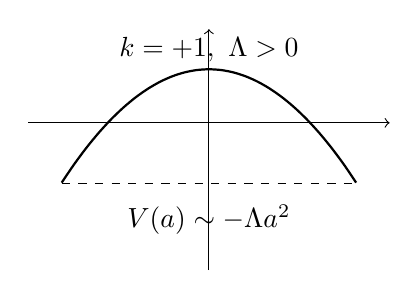
\begin{tikzpicture}[scale=0.85]
\draw[->] (-2.7,0) -- (2.7,0);
\draw[->] (0,-2.2) -- (0,1.4);
\draw[thick,domain=-2.2:2.2,smooth] plot (\x,{-0.35*(\x)^2 + 0.8});
\draw[dashed] (-2.2,-0.9) -- (2.2,-0.9);
\node at (0,-1.45) {\(V(a)\sim -\Lambda a^2\)};
\node at (0,1.1) {\(k=+1,\ \Lambda>0\)};
\end{tikzpicture}
\hspace{2em}
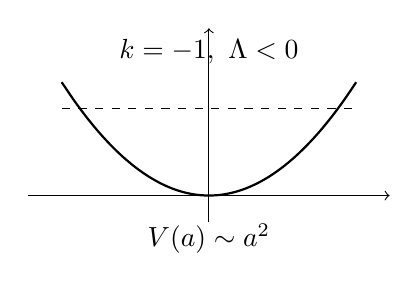
\begin{tikzpicture}[scale=0.85]
\draw[->] (-2.7,0) -- (2.7,0);
\draw[->] (0,-0.4) -- (0,2.5);
\draw[thick,domain=-2.2:2.2,smooth] plot (\x,{0.35*(\x)^2});
\draw[dashed] (-2.2,1.3) -- (2.2,1.3);
\node at (0,-0.65) {\(V(a)\sim a^2\)};
\node at (0,2.15) {\(k=-1,\ \Lambda<0\)};
\end{tikzpicture}
\caption{Schematic effective potentials for the closed de Sitter bounce and the open negative-\(\Lambda\) recollapse.}
\label{fig:c05-mechanical-potentials}
\end{figure}

\begin{classroomqa}
\audiencequestion{Are these Friedmann equations really Einstein's equations?}
\lecturerresponse{Yes. They are Einstein's field equation after homogeneity and isotropy reduce the metric to the single function \(a(t)\). The symmetry reduction removes most tensor components, leaving this ordinary differential equation for cosmic expansion. \lecturetimestamp{01:43:52--01:44:05}}
\end{classroomqa}

\begin{classroomqa}
\audiencequestion{Could the scale factor \(a\) be complex?}
\lecturerresponse{Not in the real classical FRW cosmologies being analyzed here. The scale factor measures spatial size and is taken to be real and nonnegative. Complexified geometries can appear in other mathematical approaches, but they have no role in this lecture's solutions. \lecturetimestamp{01:44:06--01:44:21}}
\end{classroomqa}

\begin{classroomqa}
\audiencequestion{Is there a physical reason pressure must be a linear function of density?}
\lecturerresponse{No. Constant \(w\) is convenient and happens to describe the principal components considered here. A mixture of matter, radiation, and vacuum does not have one constant \(w\) over all epochs, and a general material can have nonlinear \(P(\rho)\). For a barotropic fluid, \(dP/d\rho\) controls the squared sound speed in units with \(c=1\); constant \(w\) makes that derivative constant, but nature is not obliged to do so. \lecturetimestamp{01:44:21--01:45:34}}
\end{classroomqa}

\section{What to Carry Forward}

The equation of state connects microscopic physics with the time history of the scale factor. Adiabatic work in a comoving box gives
\[
\rho\propto a^{-3(1+w)}.
\]
Cold matter has \(w=0\) and \(\rho\propto a^{-3}\). Isotropic photon momentum flow gives
\[
\left\langle\cos^2\theta\right\rangle=\frac13,
\qquad
P_{\mathrm r}=\frac{\rho_{\mathrm r}}{3},
\qquad
\rho_{\mathrm r}\propto a^{-4}.
\]

Tension makes negative pressure physically intelligible. A constant vacuum density obeys
\[
P_\Lambda=-\rho_\Lambda,
\qquad
w_\Lambda=-1.
\]
Positive vacuum energy gives exponential de Sitter expansion in flat slicing and a \(\cosh\) bounce in closed slicing. Negative vacuum energy can make even an open universe recollapse. In every sign case, the Friedmann equation can be read as an effective mechanical energy equation. The unresolved question is not why quantum fields contribute vacuum energy, but why their observed net contribution is almost zero without being exactly zero.
